\documentclass[a4paper,12pt, oneside]{article}
\usepackage[utf8]{inputenc}
\usepackage[english]{babel}
\usepackage{fancyhdr}
\usepackage{geometry}
\usepackage{graphicx}
\usepackage{float} 
\usepackage{epstopdf}
\usepackage{amsmath}
\usepackage{amssymb}
\usepackage{siunitx}
\usepackage{enumitem}
\usepackage{booktabs}
\usepackage{gensymb}
\usepackage{makecell}
\usepackage{indentfirst}
\usepackage{bigints}
\usepackage{esint}
\usepackage{harpoon}
\usepackage{relsize}
\usepackage{cite}
% \usepackage{natbib}

\usepackage{subfig}
\usepackage{overpic}

\geometry{a4paper,scale = 0.8}
\pagestyle{fancy}
\fancyhead[R]{Gauss~\textsc{Chang} \\ Department of Physics, NTU}
\fancyhead[L]{\textsc{Deep Learning Based \\ Seismic Wave Identification}}
\fancyfoot[C]{\thepage}

\setlength{\parindent}{2em}

\renewcommand{\headrulewidth}{2pt}
\renewcommand{\footrulewidth}{1pt}
% \renewcommand\thesection{\arabic {section}}
\renewcommand\thesection{\Roman{section}}
\renewcommand{\thesubsection}{\thesection.\Roman{subsection}}
\newcommand{\HRule}{\rule{\linewidth}{2pt}}

%[Lenny]
% \ChNameUpperCase
% \ChNumVar{\fontsize{80}{42}\usefont{OT1}{ptm}{m}{n}\selectfont}
% \ChTitleVar{\Huge\sc}
% \ChRuleWidth{2pt}

%Make Chapter header and footer
\makeatletter
\let\ps@plain\ps@fancy
\makeatother


%Package and definition for code demo
\usepackage{listings}
\usepackage{color}
\definecolor{dkgreen}{rgb}{0,0.6,0}
\definecolor{gray}{rgb}{0.5,0.5,0.5}
\definecolor{mauve}{rgb}{0.58,0,0.82}
\lstset{frame=single,
language=Python,
aboveskip=3mm,
belowskip=3mm,
showstringspaces=false,
columns=flexible,
basicstyle={\small\ttfamily},
numbers=left,
numberstyle=\tiny\color{gray},
keywordstyle=\color{blue},
commentstyle=\color{dkgreen},
stringstyle=\color{mauve},
breaklines=true,
breakatwhitespace=true,
tabsize=4}

% \begin{enumerate} [label = (\alph*)]
% \begin{enumerate} [label = (\roman*)]
\linespread{1.5}
\begin{document}

%---------------------------Titlepage---------------------------

\begin{titlepage}

\begin{center}


% Upper part of the page

\includegraphics[width = 0.30\textwidth]{IES_logo.pdf} \\ [1cm]
% 
\includegraphics[width = 0.15\textwidth]{NTU_logo_st.pdf} \\ [1cm]
\textsc{\LARGE Institute of Earth Sciences \\ Academia Sinica} \\ [1.5cm]
\textsc{\Large Summer Internship Program} \\ [0.5cm]


% Title
\HRule \\ % [0.5cm]
{\huge \bfseries Deep Learning Based \\ Seismic Wave Identification} \\ [0.5cm]
\HRule \\ [2.5cm]

% Author and supervisor
\begin{minipage}[t]{0.4\textwidth}
\begin{flushleft} \large
\emph{Author :}\\
Gauss~\textsc{Chang} \\
% Department of Physics, NTU
\end{flushleft}
\end{minipage}
%
\begin{minipage}[t]{0.4\textwidth}
\begin{flushright} \large
\emph{Advisor :} \\
Dr.~Kuo-Fong \textsc{Ma} \\
Dr.~Wen-Tzong \textsc{Liang} \\
\end{flushright}
\end{minipage}

\vfill

% Bottom of the page
{\large \today}

\end{center}

\end{titlepage}
\setcounter{page}{1}

% \begin{enumerate} [label = (\alph*)]
% \begin{enumerate} [label = (\roman*)]

%---------------------------Body---------------------------
\abstract{Abstract}
Taiwan is a region frequently hit by earthquakes and has a dense population. This situation exerts significant pressure on structural facilities and the earthquake early warning systems. To achieve more timely earthquake warnings and post-seismic structural integrity analysis, we collaborate with QSIS in this project. Our aim is to promptly collect earthquake signals while avoiding the pitfalls of the traditional STA/LTA method \cite{app10082919}, which is prone to false activations \cite{10.1785/0220220322} \cite{10.1785/0120180080}.

\section{Introduction}
Taiwan is a region characterized by frequent earthquakes and a dense population. These conditions place immense pressure on building structures and earthquake early warning systems. In pursuit of earthquake early warning and post-quake structural integrity analysis, we introduce ``QSIS''. Harnessing the power of deep-learning, we present an affordable solution for earthquake detection. This project is meant to be:
\begin{enumerate} [label = \arabic*.]
	\item Cost-Efficient Alerts: Using MEMS technology, we can widely distribute the sensor at low costs.
	\item Instantaneous Detection: Real-time alerts for swift precautionary actions.
	\item Widespread Coverage: Designed for city-wide deployment to ensure comprehensive safety.
	\item Customization: Fine-tuning capabilities to cater to unique building or location requirements.
	\item Structural Integrity Monitoring: For different floors in a single building, identify the damaged ones using the waveform.
\end{enumerate}
%
\begin{figure}[H]
\centering
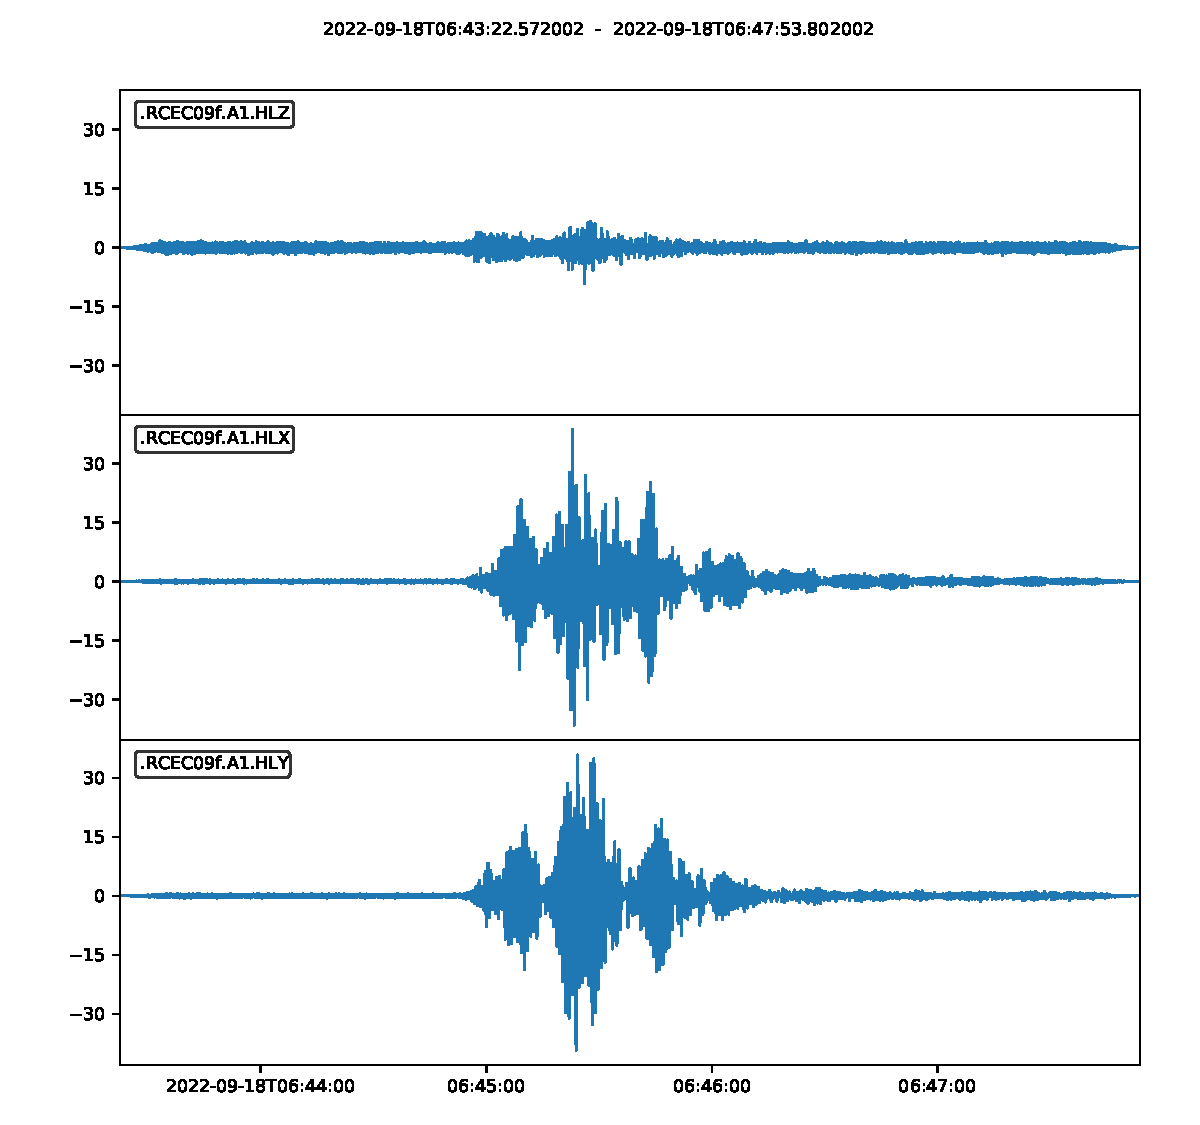
\includegraphics[width = 3in]{event_threechannel.pdf}
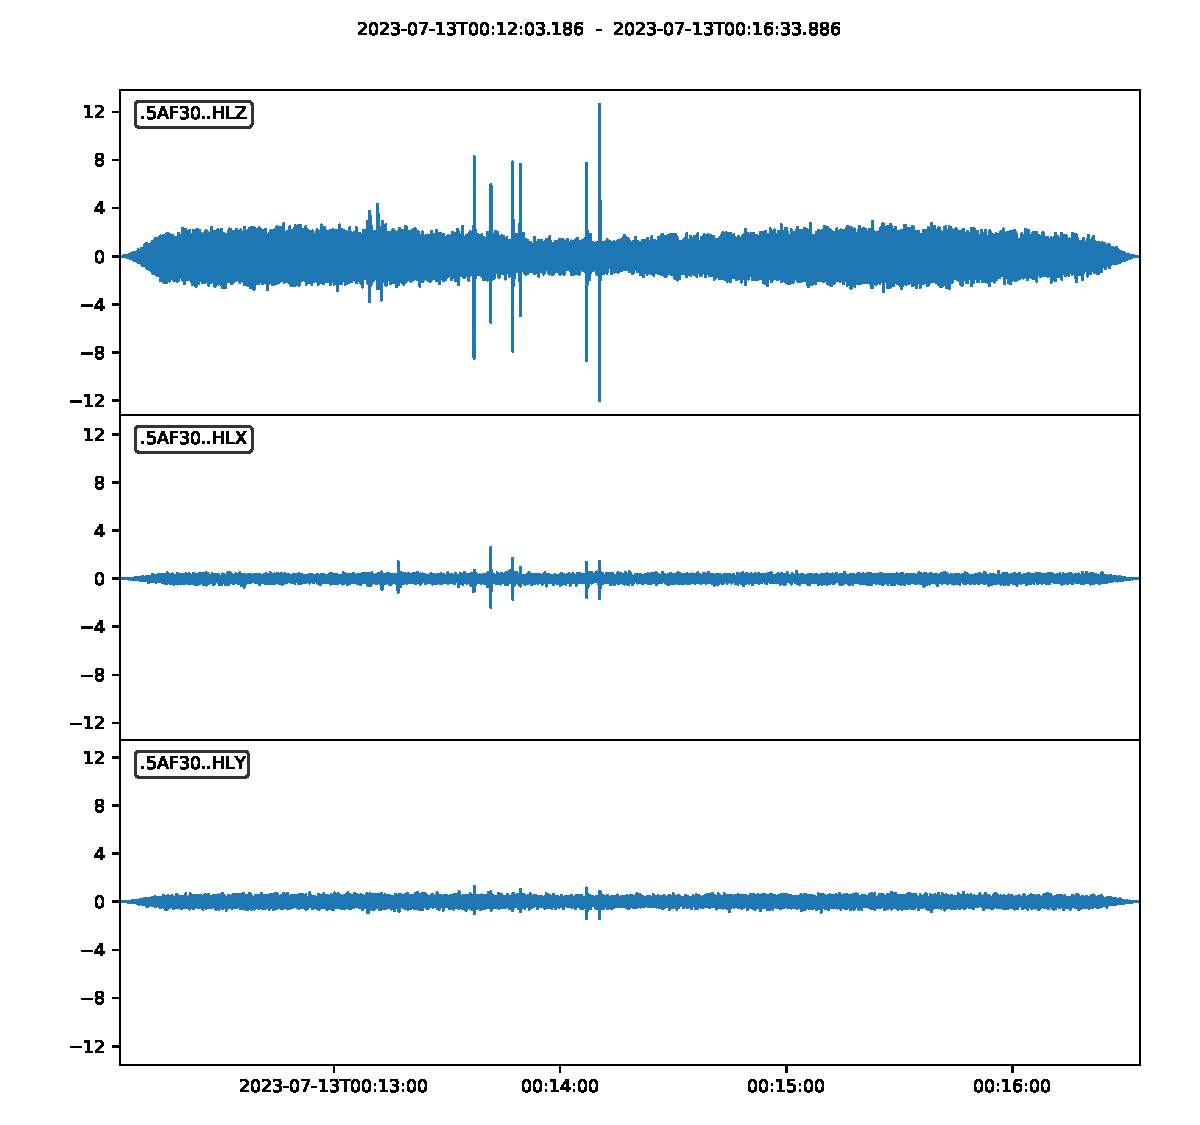
\includegraphics[width = 3in]{noise_threechannel.pdf}
\caption{Seismic and Noise Waveform}\label{threechannel}
\end{figure}

In Figure \ref{threechannel} shows how the seismic and noise waveform look like.
%
\newpage
\subsection{Importance of this Work}
%
\newpage
\subsection{Model Structure}
Following is a model structure I have used in this project.
\begin{figure}[H]
\centering
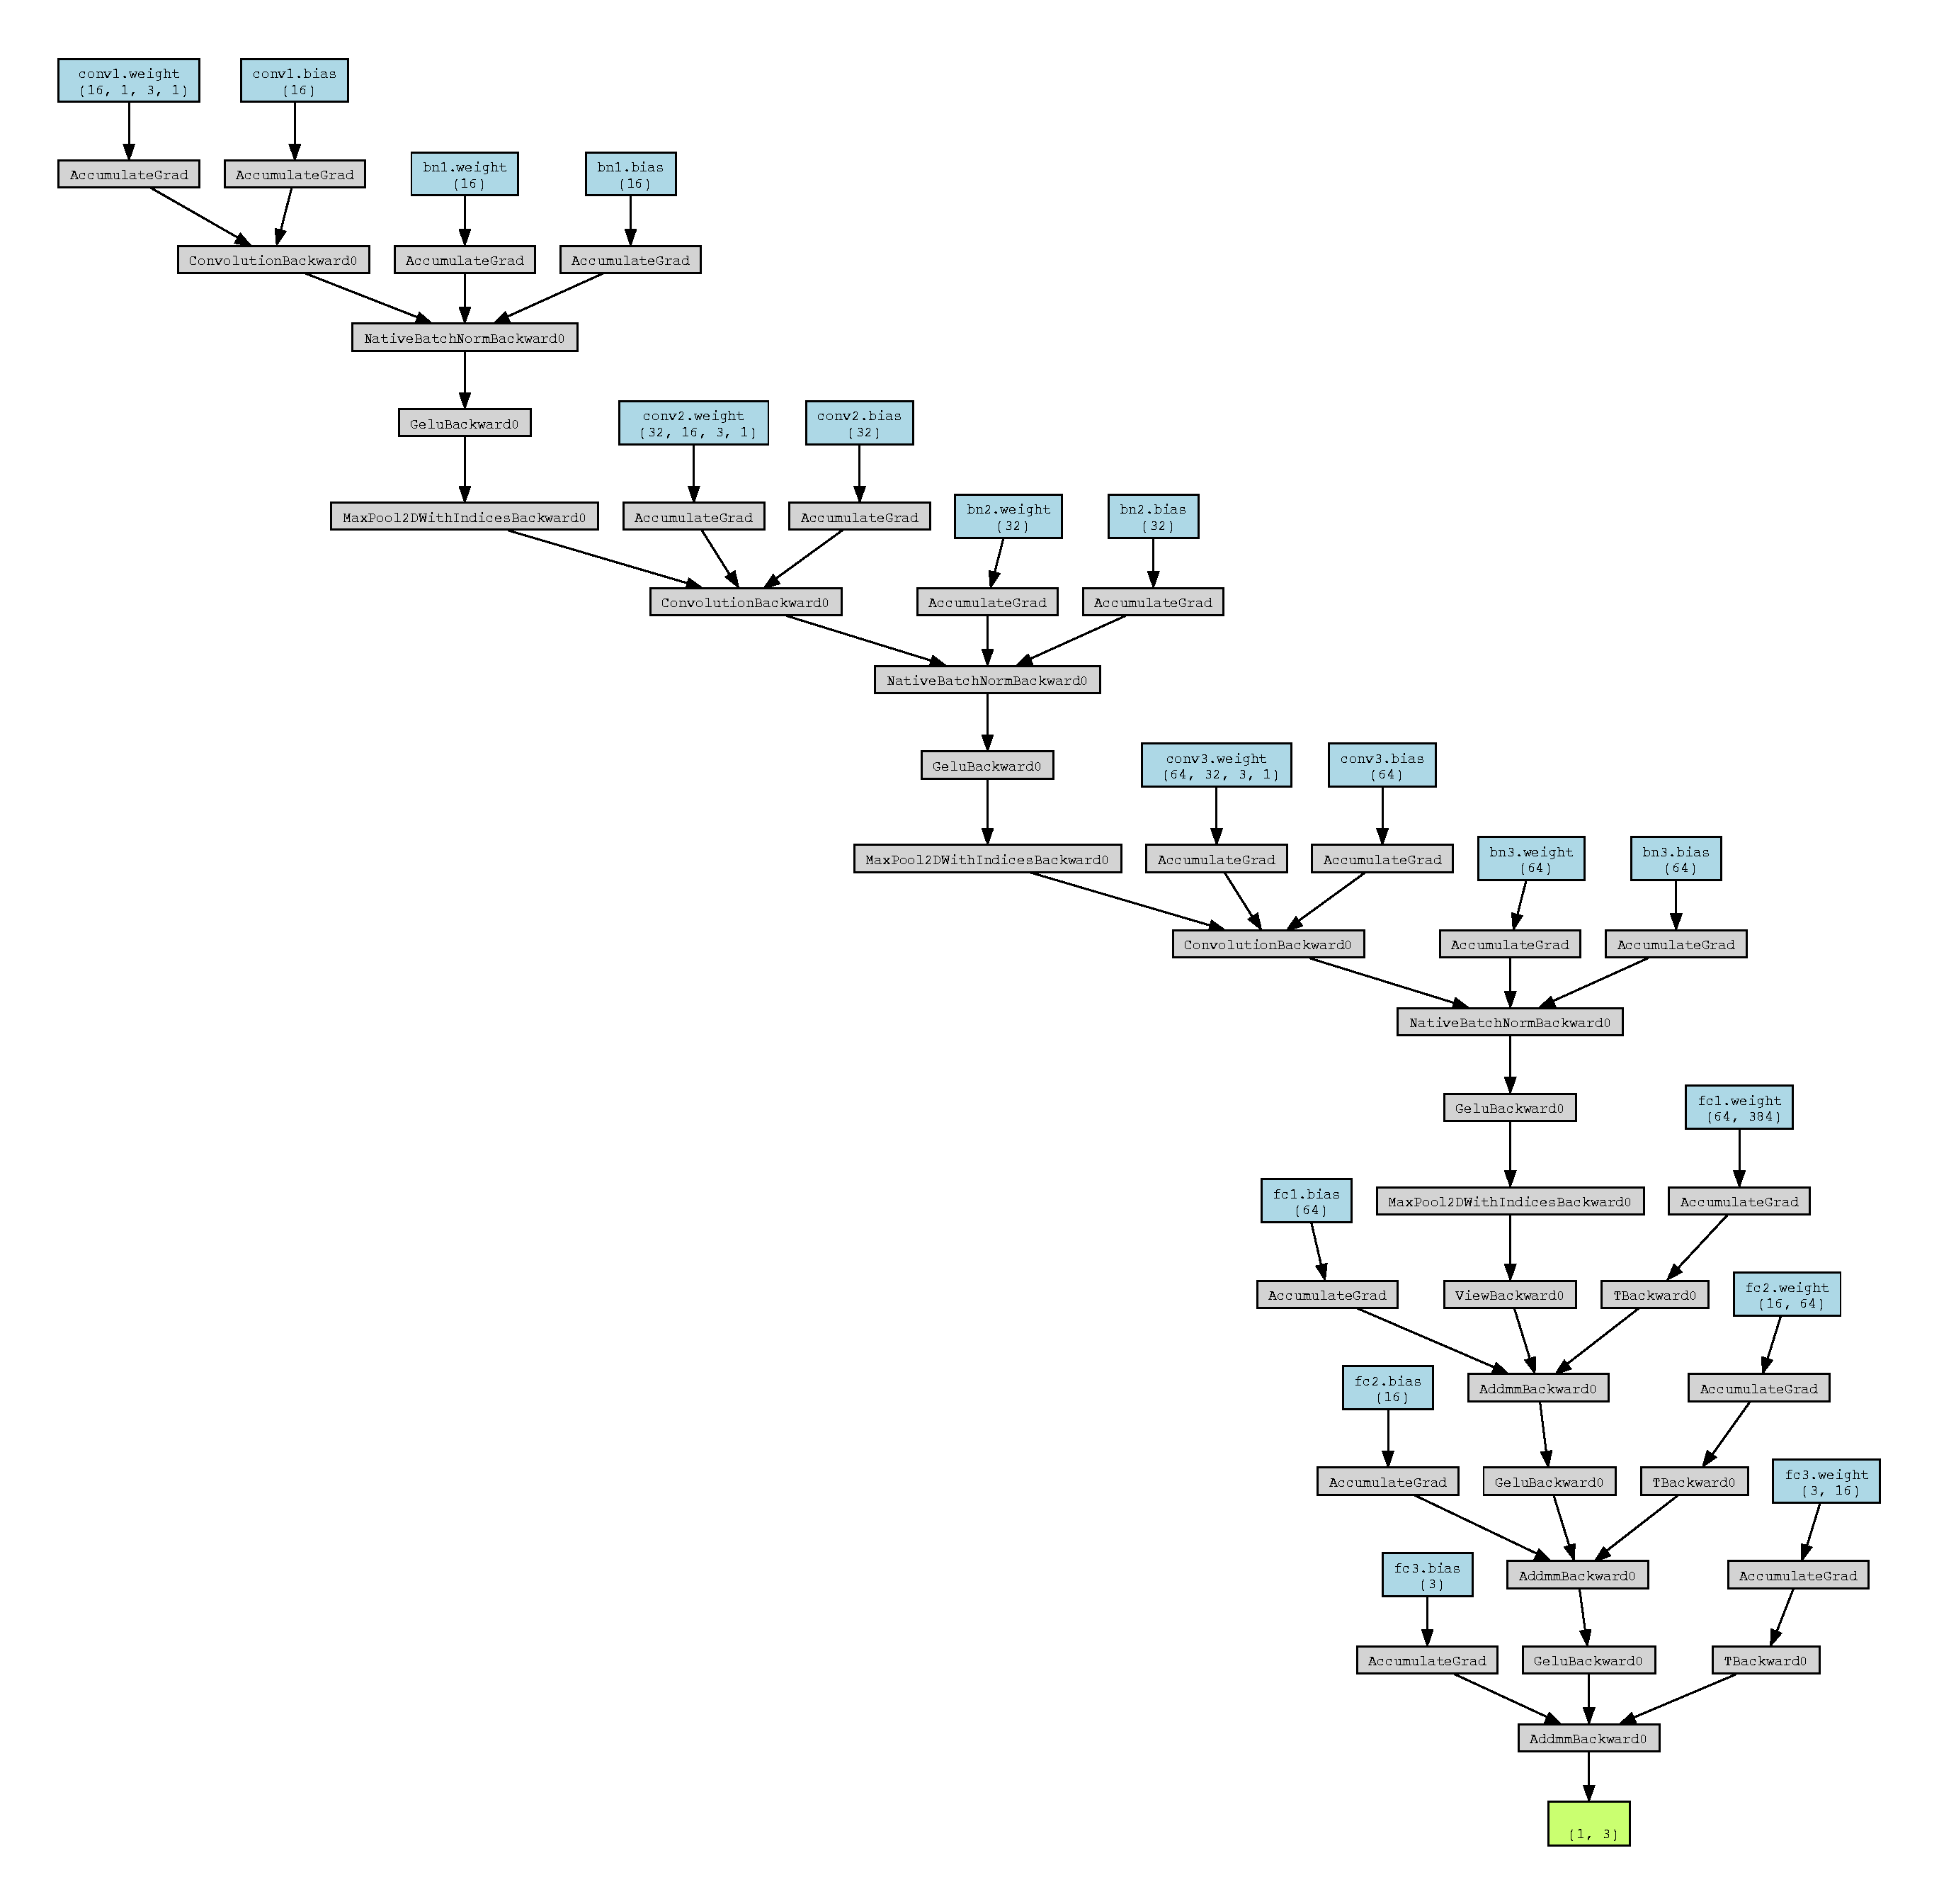
\includegraphics[width = 6in]{EarthquakeCNN_Model.pdf}
\caption{Model Structure}\label{EarthquakeCNN_Model_Structure}
\end{figure}
\newpage
\section{Training Data Structure}

Given that the QSIS project is still in its early stages, its earthquake information is somewhat lacking compared to more established databases. Therefore, for this initiative, we utilized two databases for training. Initially, we pre-trained our model using data from the STanford EArthquake Dataset (STEAD) \cite{8871127}.

The STEAD database contains 73,582 usable noise and event recordings, divided approximately into 40\% Noise, 30\% P-waves, and 30\% S-waves.

Building on this, we fine-tuned the model using the QSIS dataset, which comprises 241 usable events and 725 noise recordings. The distribution within the QSIS dataset is approximately 60\% Noise, 20\% P-waves, and 20\% S-waves.

Figures \ref{spectrogram} showcase the spectrogram from the QSIS dataset for two different buildings: IES and RCEC. As observed from the diagrams, the earthquake data recorded by IES predominantly has wave durations around \SI{4}{\hertz}, whereas the data recorded by RCEC mostly centers around \SI{1.3}{\hertz}. This suggests that earthquake signals within buildings are highly building- dependent.

\begin{figure}[H]
\centering
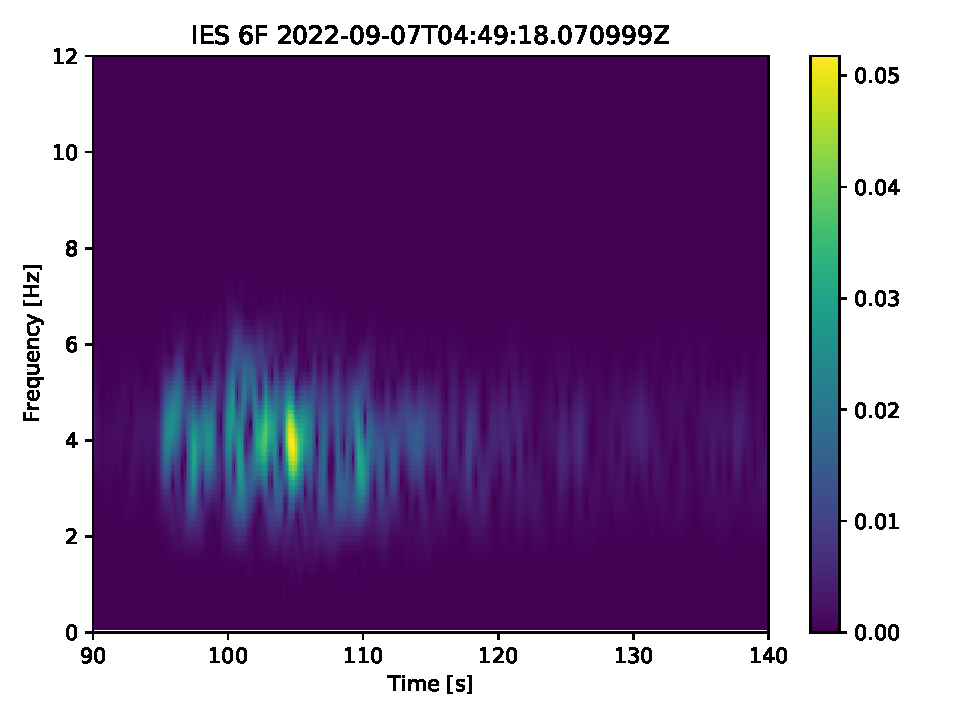
\includegraphics[width = 3in]{Single_IES_spectrogram.pdf}
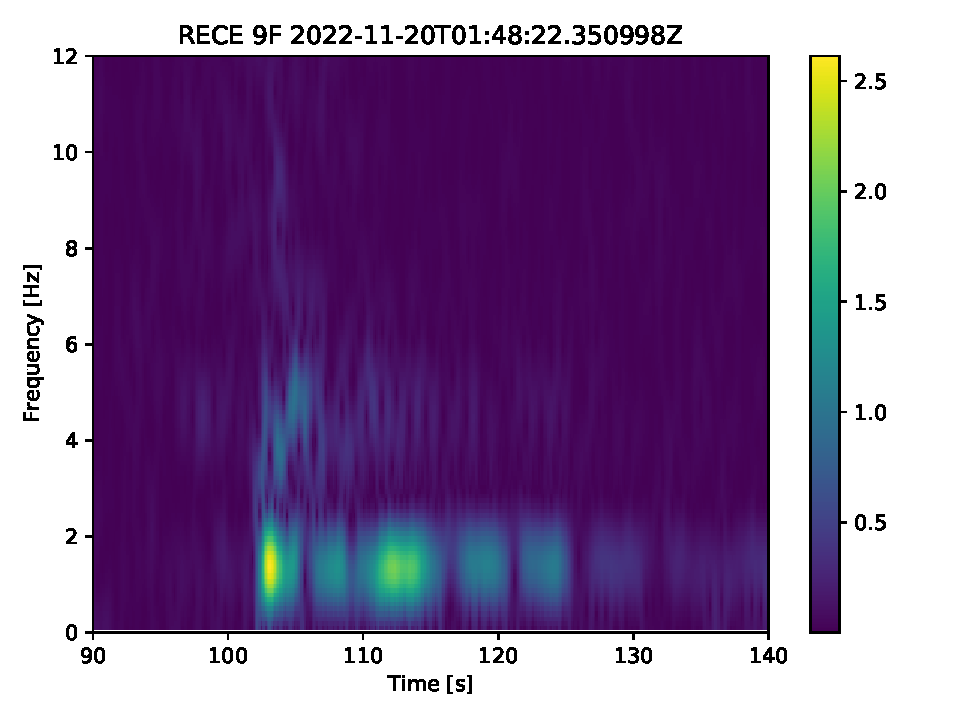
\includegraphics[width = 3in]{Single_RCEC_spectrogram.pdf}
\caption{Spectrogram of Training Data}\label{spectrogram}
\end{figure}

\newpage
\section{Implementation}
%
\newpage
%
\section{Result}
\begin{figure}[htbp]
	\centering
	\subfloat[2022-09-18 06:44:15(UTC), $23.14^{\circ}$N, $121.2^{\circ}$E, depth: 7km, ML:6.8]{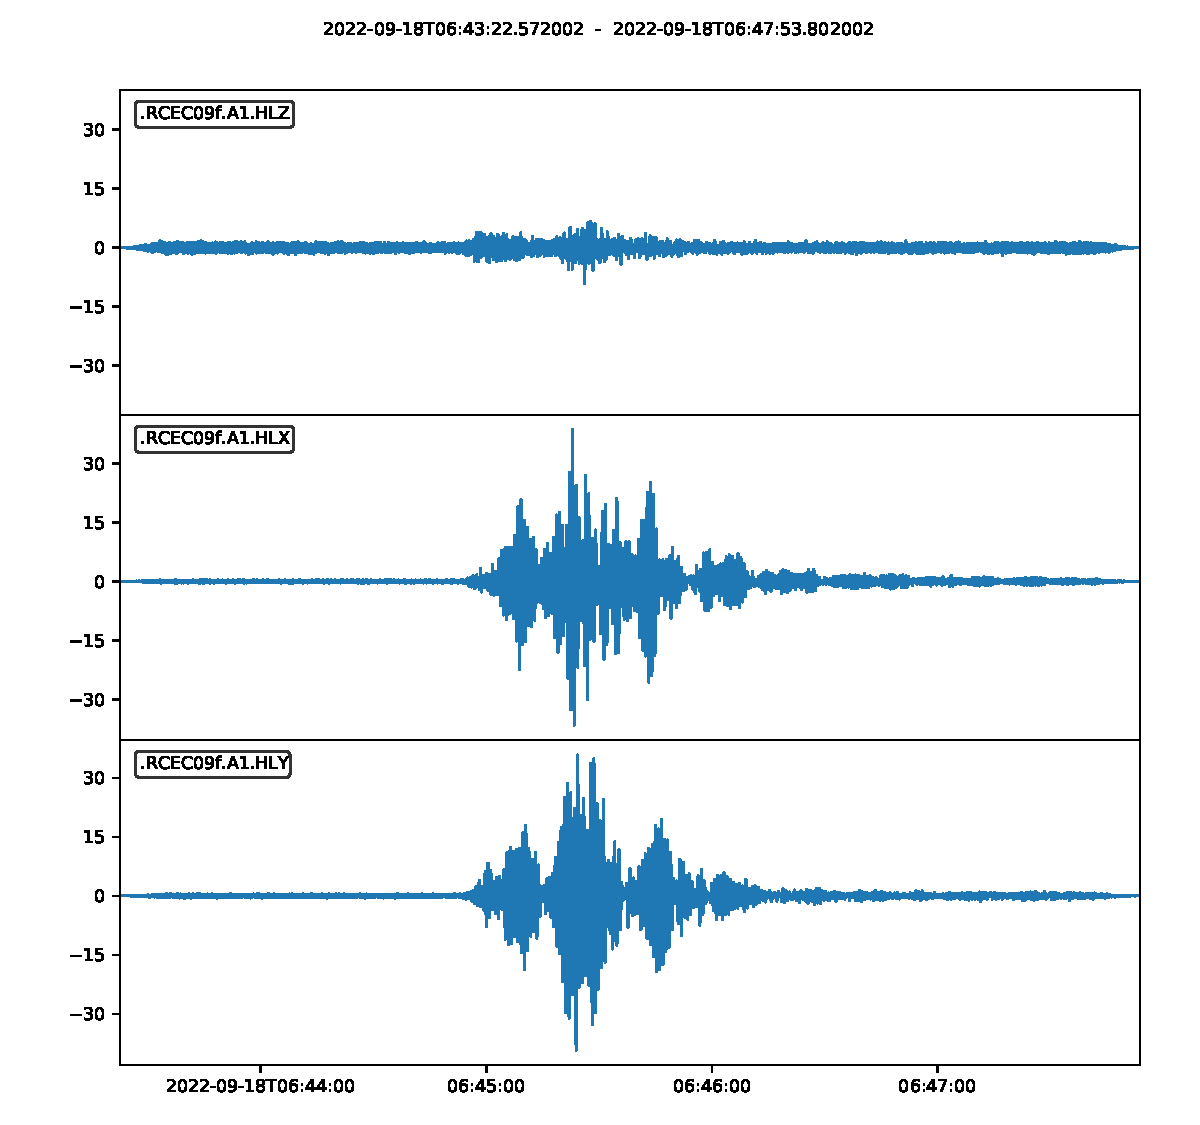
\includegraphics[width=.45\columnwidth]{./event_threechannel.pdf}}\hspace{5pt}
	\subfloat[2023-07-05 02:21:21(UTC)]{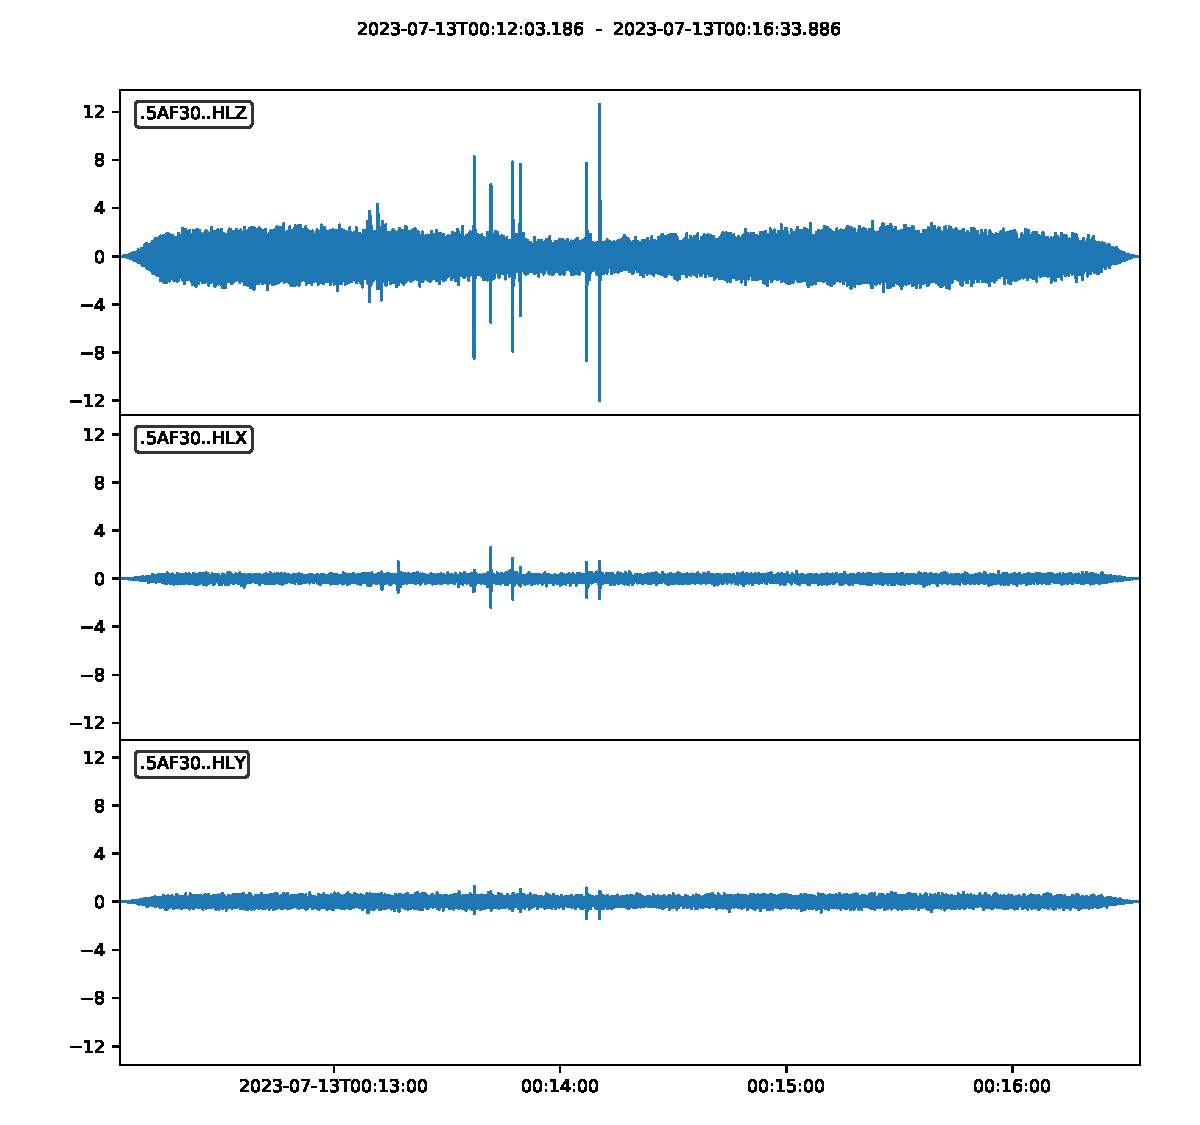
\includegraphics[width=.45\columnwidth]{./noise_threechannel.pdf}}\\
	\subfloat[Prediction of an Actual Event]{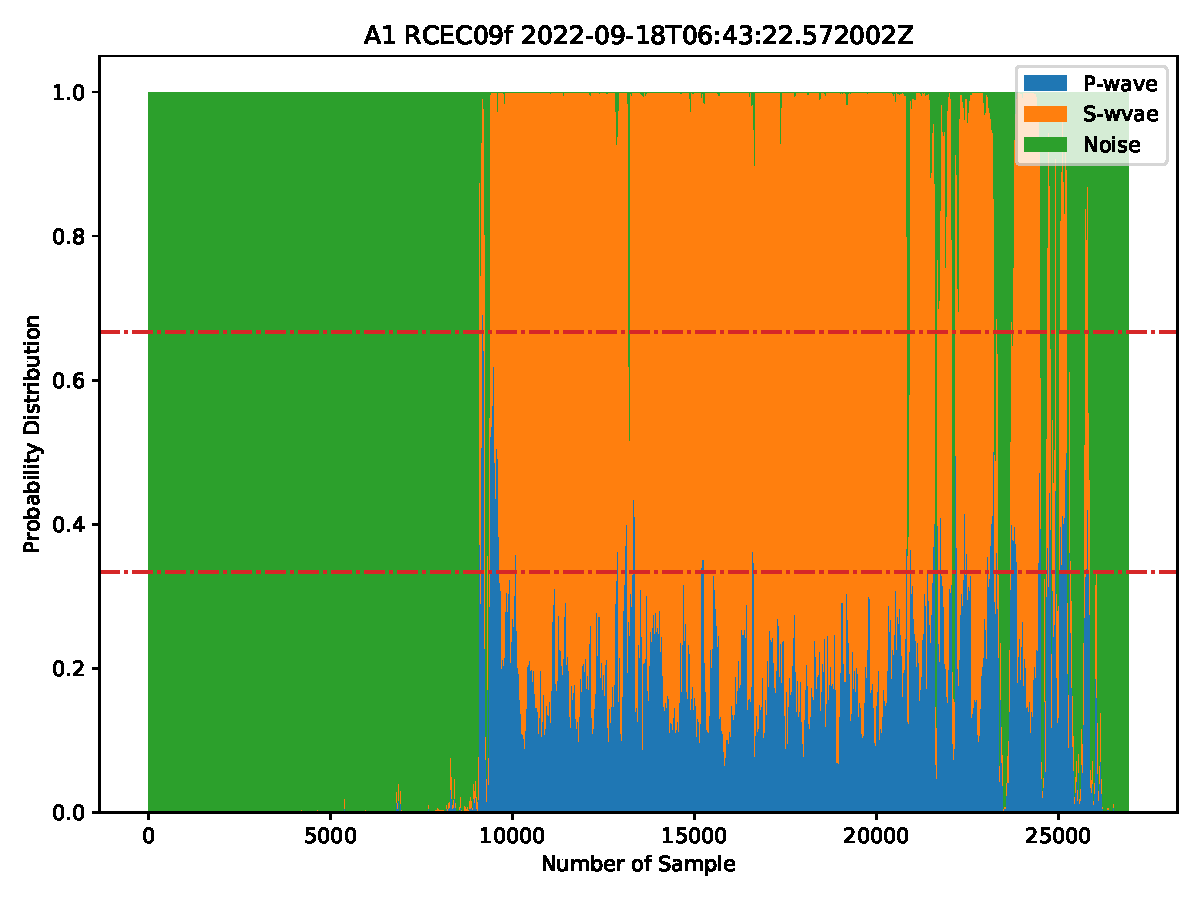
\includegraphics[width=.45\columnwidth]{./Single_event_test.pdf}}\hspace{5pt}
	\subfloat[Prediction of an Actual Noise]{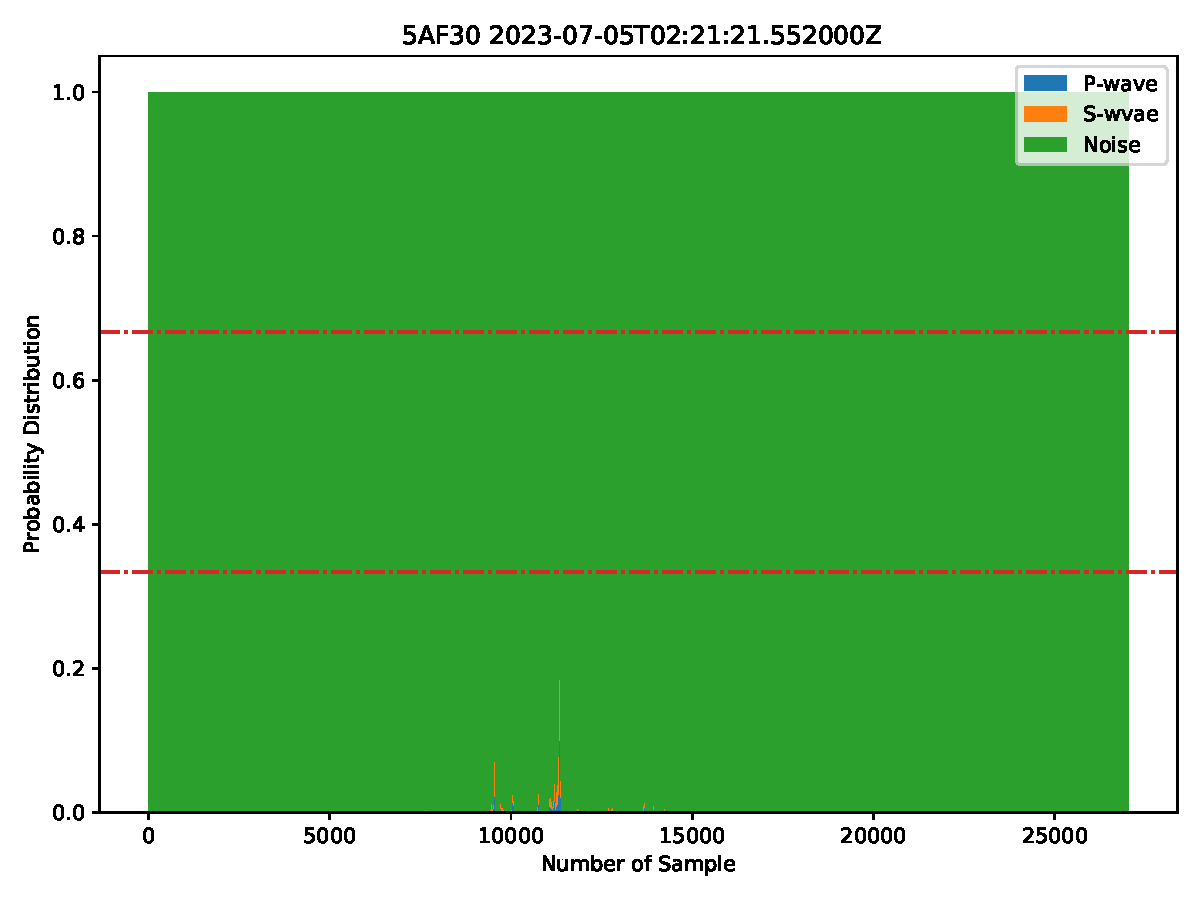
\includegraphics[width=.45\columnwidth]{./Single_noise_test.pdf}}
	\caption{Prediction Results}
\end{figure}
%
\newpage
\section{Conclusion}

\newpage
\bibliographystyle{unsrt}
\bibliography{bibliography.bib}

\end{document}



















